\section{csnap}

\subsection{csnap}
\begin{frame}[fragile]
\only<1>{
  {\Huge \texttt{csnap}}\\
  CLI, Programmiersprache C, 650 LOC
}

\only<2>{
\begin{center}
 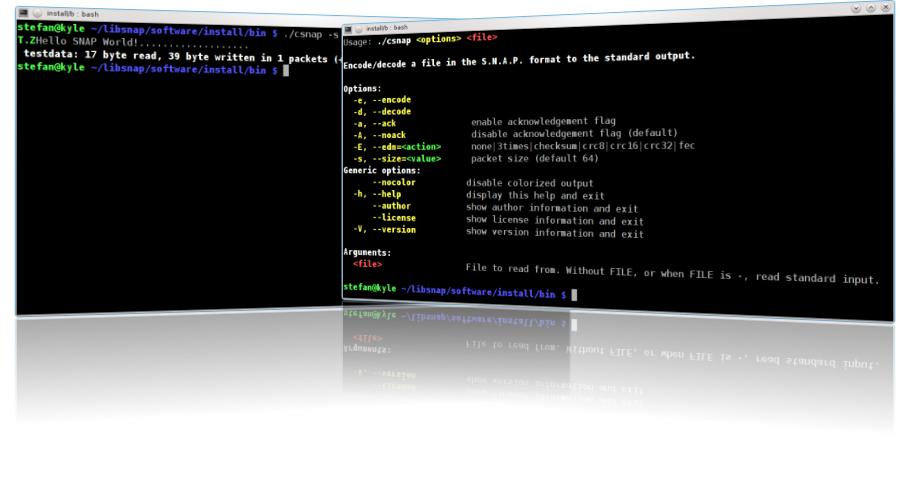
\includegraphics[scale=0.4]{images/screenie_csnap.png}
\end{center}
}
\end{frame}


\begin{frame}[fragile]
\begin{center}
 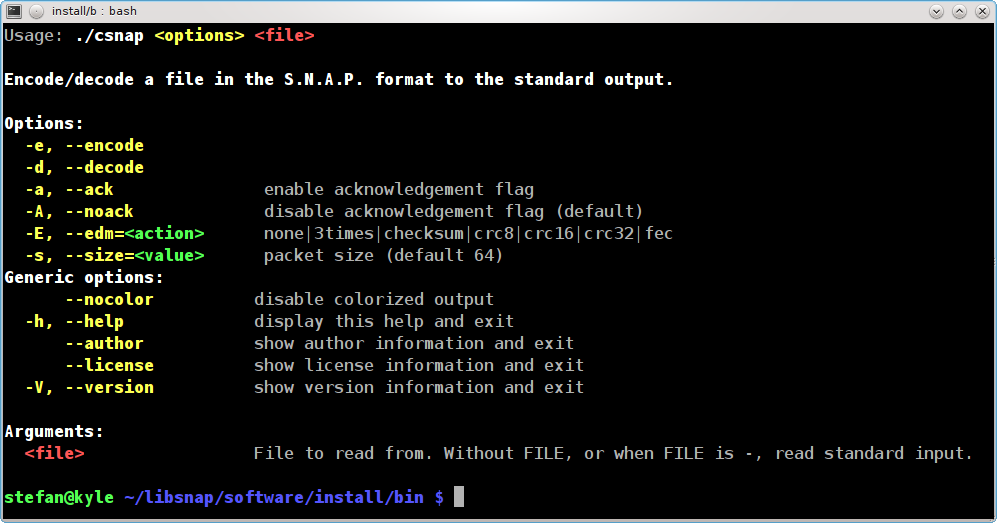
\includegraphics[scale=0.4]{images/csnap_1.png}
\end{center}
\end{frame}

\begin{frame}[fragile]
\begin{center}
 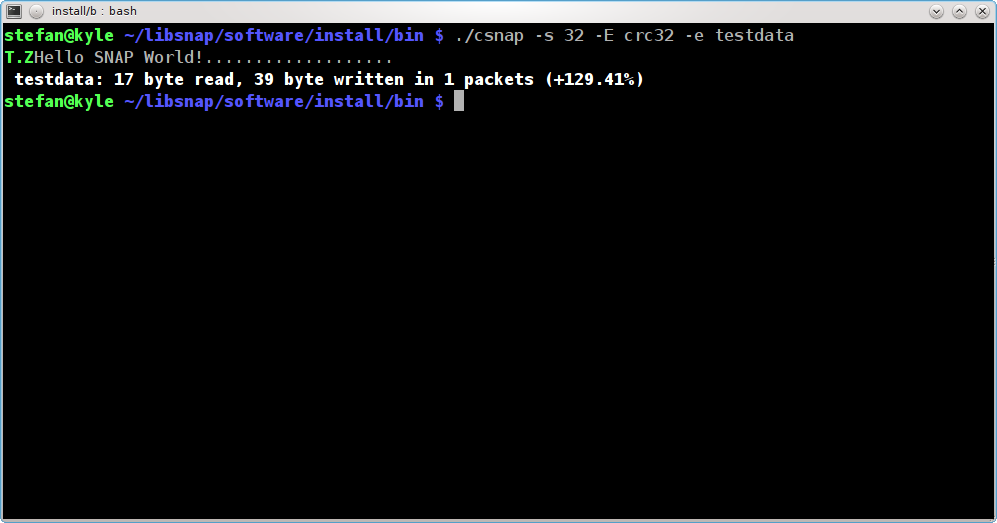
\includegraphics[scale=0.4]{images/csnap_2.png}
\end{center}
\end{frame}

\begin{frame}[fragile]
\begin{center}
 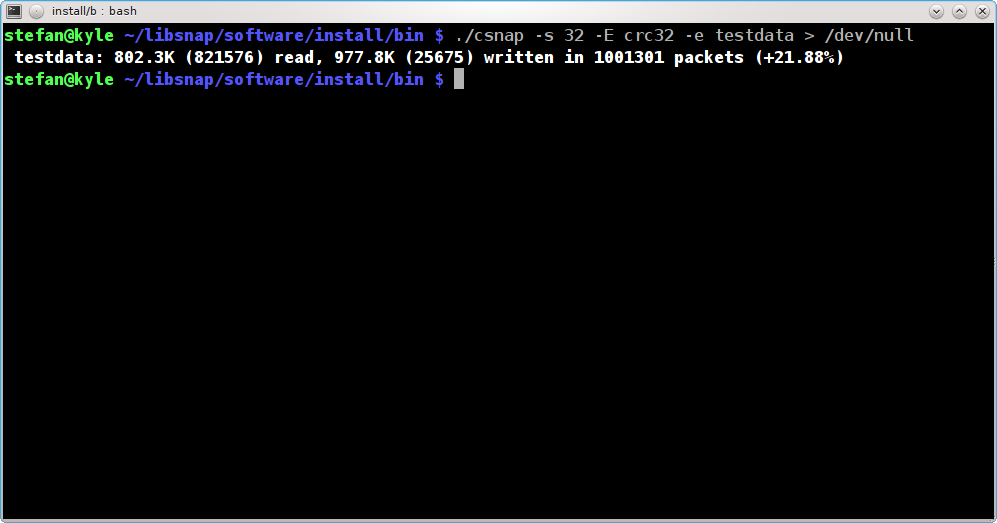
\includegraphics[scale=0.4]{images/csnap_3.png}
\end{center}
\end{frame}

% kate: word-wrap off; encoding utf-8; indent-width 4; tab-width 4; line-numbers on; mixed-indent off; remove-trailing-space-save on; replace-tabs-save on; replace-tabs on; space-indent on;
% vim:set spell et sw=4 ts=4 nowrap cino=l1,cs,U1:
